\RequirePackage{fix-cm}
\documentclass[smallextended]{svjour3}       % onecolumn (second format)
\smartqed  % flush right qed marks, e.g. at end of proof
%
%\usepackage{graphicx}

%Para funcionar o CITEP:
\usepackage[square,sort]{natbib}

%Para rodar em português com cedilha e hifenização certa.
\usepackage{graphicx,url}
\usepackage[brazil]{babel}   
\usepackage[utf8]{inputenc}  
%\usepackage[alf]{abntex2cite}

%
% Insert the name of "your journal" with
\journalname{Data Min Knowl Disc}
%
\begin{document}
	
\title{Detecção de Fraudes em Cartões de Crédito: Uma Revisão Sistemática
}
\subtitle{}

\titlerunning{Detecção de Fraudes em Cartões de Crédito: Uma Revisão Sistemática}

\author{Jean Avila Rangel         \and
	Maria Claudia Figueiredo Pereira Emer \and
	Adolfo Gustavo Serra Seca Neto
}

\institute{Jean Avila Rangel
\at Federal University of Technology - Paraná, 3165 Sete de Setembro Avenue, Curitiba, PR 80230-901, BRA
\and
Maria Claudia Figueiredo Pereira Emer \and Adolfo Gustavo Serra Seca Neto
\at Academic Department of Informatics, Federal University of Technology - Paraná, 3165 Sete de Setembro Avenue, Curitiba, PR 80230-901, BRA
\\\email{mciemer@gmail.com} 
\\
\and
Adolfo Gustavo Serra Seca Neto \\\email{adolfo@dainf.ct.utfpr.edu.br}
}
	\date{Received: date / Accepted: date}
	% The correct dates will be entered by the editor
	\maketitle
	
	\begin{abstract}
		Insert your abstract here. Include keywords, PACS and mathematical
		subject classification numbers as needed.
		\keywords{Fraud detection \and Anomaly detection \and Deception detection \and Standard deviation detection \and Detecção de fraude \and Detecção de anomalia \and Detecção de engano \and Detecção de desvio padrão}
	\end{abstract}
	
\section{Introdução}

A detecção de fraudes é utilizada para resolver problemas variados, sendo geralmente utilizada para reduzir falhas de segurança em sistemas onde há gasto de recursos com usuários mal intencionados.

Segundo \cite{Fawcett1997}, há muitas técnicas para detecção de fraudes. As mais difundidas e utilizadas são as que produzem detecções por meio de regras pré estabelecidas e as que realizam a comparação entre valores de dados. Estas classificações geraram duas principais ramificações em pesquisas.

Uma das ramificações, a detecção de fraude por meio de regras, determina que uma fraude será detectada devido ao conhecimento que a equipe adquiriu observando fraudes recorrentes em outrora. A vantagem nesta técnica está em preditar como a fraude ocorre. A desvantagem está na possibilidade de descobrir somente fraudes já conhecidas.

O outro ramo na detecção de fraudes ocorre por meio de cálculos e comparação de valores. Como principal exemplo, um desvio no padrão comportamental de alguma variável pode ser identificado comparando seus dados com dados anteriores ou de outras variáveis similares. Sua principal vantagem é a utilização de algoritmos já conhecidos na literatura \citep{Fawcett1997}. O problema apresentado pela técnica é a possibilidade do indivíduo fraudador a conhecer e inserir dados fraudulentos de maneira em que o sistema não consiga o identificar como um usuário malicioso.

\cite{Fawcett1997} realizaram uma das primeiras e principais abordagens no ramo de detecção de fraudes encontradas na literatura. Em seus estudos, analisaram e criaram um sistema para detecção de fraudes em sistemas de telecomunicação. Em seus estudos, constaram que indivíduos fraudadores estão constantemente mudando suas táticas para burlar sistemas, que devem adaptáveis às novas situações.

Em todo contexto organizacional, cada ambiente possui um tipo de tratamento e armazenamento de dados. Portanto, ambientes podem possuir dados organizados de maneira estável por induzirem normativas e tecnologias padronizadas ou fazer exatamente o contrário, possuindo dados desorganizados com poucas conexões lógicas. Portanto, abordagens gerais e adaptáveis em detecção de fraudes são esperadas para desenvolver este trabalho.

\cite{Fawcett1997} realizaram um trabalho em detecção de fraude em cartões de crédito utilizando dados reais, fornecidos por companhias bancárias, e obtiveram um aumento nos seus resultados em comparação com técnicas de detecções de fraudes utilizadas anteriormente. Em suas constatações, indicaram que os métodos mais potentes para detectar fraudes são utilizados em cartões de crédito, porém as organizações não costumam revelar suas tecnologias de forma aberta, pois possíveis fraudadores podem se aproveitar do conhecimento e utilizar nos sistemas com má fé.

A realização da revisão sistemática proposta por este trabalho obtém motivação devido à crescente expansão do Estado da Arte no assunto. Em pesquisas realizadas em bases de dados por trabalhos realizados na área de detecção de fraude, notou-se a produção de muito material anteriormente ao ano de 2010, porém com um significativo aumento na porcentagem de publicações posteriores a 2010. Este fator indica o crescimento do interesse da comunidade científica em pesquisar o assunto.

O controle organizacional de uma empresa ou setor pode garantir a sua boa estabilidade. Soluções para detectar, prevenir e evitar fraudes podem se tornar uma ferramenta para auxiliar a economia de recursos \citep{809570}. 

A detecção de fraudes vem sendo utilizada há muito tempo para controle organizacional e econômico \citep{Seyedhossein2010}. Em estudos realizados no estado da arte, houve uma grande apresentação sobre algoritmos para detectar fraudes em sistemas financeiros ou de cartão de crédito \citep{809570}, \citep{Chandola:2009:ADS:1541880.1541882} e \citep{Abdallah201690}.

O problema computacional que ainda ocorre é a não detecção de todos os falsos negativos (onde ações fraudulentas não são detectadas), bem como a classificação equivocada de falsos positivos (ações legítimas caracterizadas, erroneamente, como fraudulentas). Identificar uma forma para reduzir a incidência de erros é uma importante contribuição para a área e a principal justificativa para este estudo. 

O objeto de estudo do trabalho consiste em encontrar técnicas de detecção de fraude aplicáveis a contextos de cartões de crédito e que apresentem bons resultados e desempenho. A eficácia e utilidade dos algoritmos computacionais serão analisadas e consideradas para realizar estudos futuros onde serão aplicadas concomitantemente.

\subsection{Objetivos}

\subsubsection{Objetivo Geral}
Este trabalho possui como objetivo geral realizar uma revisão sistemática em trabalhos e técnicas voltados para detecção de fraudes. Desta forma, sistemas desenvolvidos para inspecionar desvio de padrões, comportamentos indevidos ou fraudes em cartões de crédito serão identificados e estudados através dos trabalhos publicados no Estado da Arte.

\subsubsection{Objetivos Específicos}

Para encaixar o objeto que está sendo estudado com o problema apresentado, pretende-se - após realizada a pesquisa entre trabalhos na área - encontrar uma ou um conjunto de técnicas apropriadas para resolver o problema computacional apresentado.

Paralelamente com o objetivo geral, espera-se encontrar as carências que os trabalhos estudados demonstram. As falhas cometidas por autores passados sobre o assunto podem gerar novas pesquisas e um melhor aprofundamento sobre o tema. 

Também se espera realizar uma revisão sistemática considerando os trabalhos que foram publicados após as ultimas revisões sistemáticas serem escritas.

Todas as técnicas para detecção de fraudes que forem encontradas e consideradas relevantes serão apresentadas e descritas.

\section{Materiais e Métodos de Pesquisa}
\label{sec:1}

Ao primeiro momento do trabalho de revisão sistemática, o planejamento da estratégia de pesquisa norteia a pesquisa em publicações na área abordada.

A revisão da literatura foi baseada no trabalho apresentado por \cite{Kitchenham07guidelinesfor}, onde os elementos de pesquisa são definidos para realizar e relatar a revisão.

Foram selecionadas as bibliotecas digitais abaixo para realizar a pesquisa. O motivo da escolha foi a grande quantidade de material publicado com relevância científica.

\begin{itemize}
	\item \textsf{ACM Digital Library}\index{ACM Digital Library}\footnote{\url{http://dl.acm.org/}}
	
	\item \textsf{IEEE Xplore Digital Library}\index{IEEE Xplore Digital Library}\footnote{\url{http://ieeexplore.ieee.org/}}
	
	\item \textsf{ScienceDirect}\index{ScienceDirect}\footnote{\url{http://www.sciencedirect.com/}} 	
	
	\item \textsf{SpringerLink}\index{SpringerLink}\footnote{\url{http://link.springer.com/}}
\end{itemize}

A tarefa para selecionar os artigos pode ser visualizada no diagrama da Figura \ref{fig:diagrama}, onde as etapas foram divididas em início, desenvolvimento e conclusão. Na parte inicial, o tema é definido e publicações naquele tema são pesquisadas. 

\begin{figure}[!ht]
	\centering
	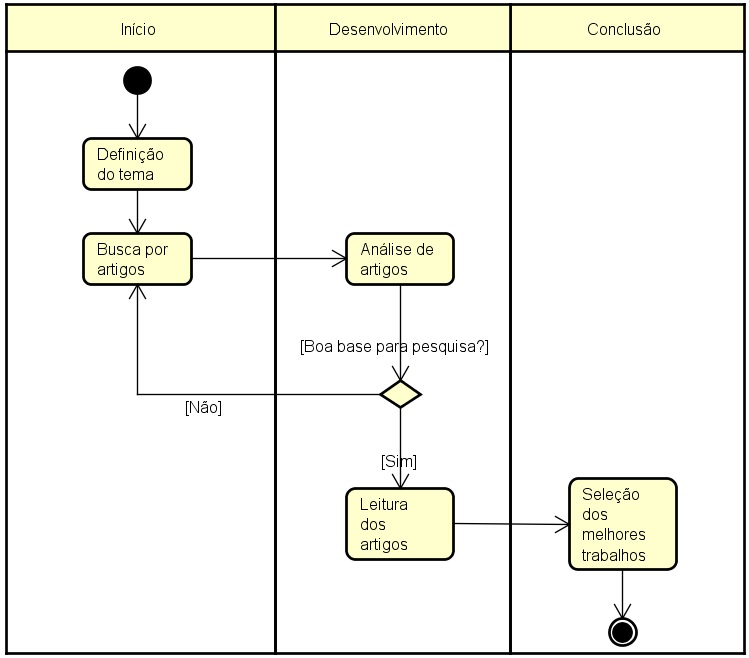
\includegraphics[width=0.9\textwidth]{imagens/diagrama.jpg}
	\caption{Diagrama de sequência indicando as etapas da pesquisa.}
	\label{fig:diagrama}
\end{figure}

Para a busca de publicações, foram considerados somente trabalhos na língua inglesa e publicados no período entre 2006 e 2016. As palavras chave \emph{credit card fraud detection} foram utilizadas para a busca, que obteve artigos selecionados com a leitura na respectiva ordem: título, resumo e artigo completo. 

Como critérios de seleção, a revisão teve como critério de escolha os artigos com maior número de citações e relevância para a área. Realizando uma exceção temporal, os principais artigos foram inclusos no estudo, pois eram encontrados como referência na maioria dos trabalhos atuais.

Outro critério de seleção foi a proximidade com o tema destacado na introdução deste trabalho, onde a detecção de fraudes ocorridas em cartões de crédito deveria ser a principal abordagem do artigo encontrado.

Foram excluídos da revisão os artigos que fugiam do tema proposto, não possuíam citações ou relevância nas bases de dados ou eram anteriores ao ano de 2006.

Após os artigos serem analisados, caso se encontre pouca base para a pesquisa, a tarefa de busca por artigos é refeita e somente após a estabilização de uma boa base para pesquisa, os trabalhos são estudados e os melhores são elencados.

\section{Cronograma}
\label{sec:4}

Conforme visto na Figura \ref{fig:cronograma}, o escopo do trabalho foi delimitado pelas tarefas: Definir tema; Definir objetivos, justificativa e motivação; Escolher o local para publicação; Elaborar o método de pesquisa; Revisar a literatura e selecionar trabalhos; Produzir artigo científico; e Publicar o artigo finalizado. 

As tarefas foram divididas entre os meses de junho a setembro e receberam a classificação: Concluída ("OK", em verde); Em andamento ("Andam.", em amarelo); e Não iniciada ("Não Inic.", em vermelho). 

\begin{figure}[!ht]
	\centering
	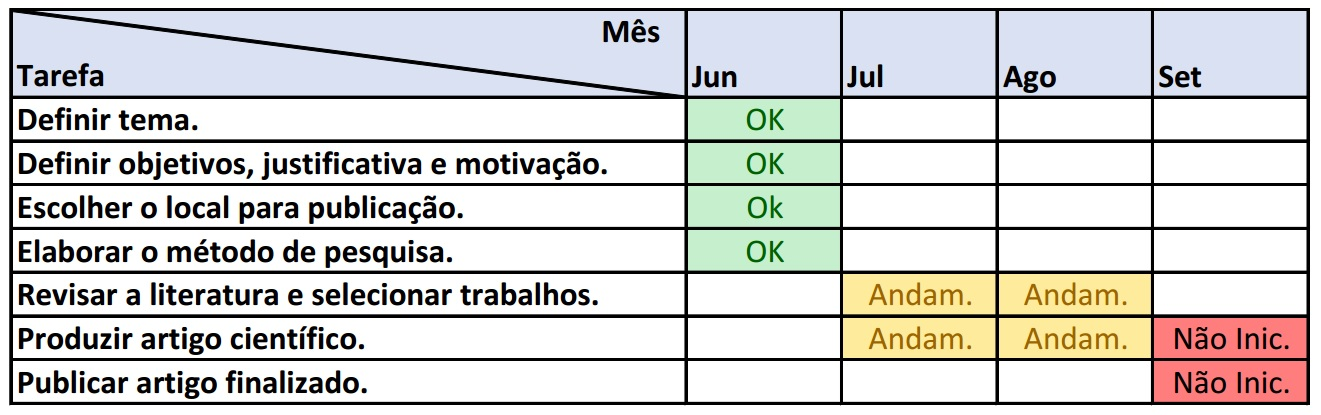
\includegraphics[width=1\textwidth]{imagens/cronograma2.jpg}
	\caption{Cronograma do planejamento do projeto.}
	\label{fig:cronograma}
\end{figure}
	
\section{Projeto de Pesquisa do Mestrado}
\label{sec:5}

Na finalização da revisão sistemática, espera-se a publicação dos resultados obtidos na revista Data Mining and Knowledge Discovery, a qual possui a classificação de qualidade Qualis B1, elencada pela CAPES em sua última análise. 

	% BibTeX users please use one of
	\bibliographystyle{spbasic}      % basic style, author-year citations
	%\bibliographystyle{spmpsci}      % mathematics and physical sciences
	%\bibliographystyle{spphys}       % APS-like style for physics
	\bibliography{minhabibliografia}   % name your BibTeX data base
	
\end{document}